\documentclass[10pt, letterpaper]{paper}
\usepackage{graphicx}
\usepackage{amsmath}
\usepackage{float}

\title{ Operations Research HW2 }
\author{ Timothy Schwieg }
\date{ September 12 2017 }

\begin{document}

\maketitle

\section*{Question 1 }
\subsection*{a.}
\begin{equation*}
\begin{alignedat}{3}
&\text{max }&-2x_1 + 5x_2 - 6x_3 + 6a_1&\\
&\text{s.t. } &3x_1 + 7x_2 + x_3 - a_1 + s_1 &= 1 \\
& &-5x_1 = 3x_2 - x_3 + a_1 - s_2 &= 10\\
& &2x_1 + 5x_2 &= 12\\
& &x_1, x_2, x_3, s_1, s_2, a_1 &\geq 0
\end{alignedat}
\end{equation*}

\subsection*{b.}
If the objective function is changed to max $z = 2x_1 - 5x_2 + 6x_3$ This is equivalent to: $min z = -2x_1 + 5x_2 - 6x_3$
So our linear program in standard form becomes: 
\begin{equation*}
\begin{alignedat}{3}
&\text{max }&x_1 - 5x_2 + 6x_3 - 6a_1&\\
&\text{s.t. } &3x_1 + 7x_2 + x_3 - a_1 + s_1 &= 1 \\
& &-5x_1 = 3x_2 - x_3 + a_1 - s_2 &= 10\\
& &2x_1 + 5x_2 &= 12\\
& &x_1, x_2, x_3, s_1, s_2, a_1 &\geq 0
\end{alignedat}
\end{equation*}

\subsection*{c.}
The Standard form of a the linear program changes to:
\begin{equation*}
\begin{alignedat}{3}
&\text{max }&-2x_1 + 5x_2 - 6x_3 + 6a_1&\\
&\text{s.t. } &3x_1 + 7x_2 + x_3 - a_1 + s_1 &= -1 \\
& &-5x_1 = 3x_2 - x_3 + a_1 - s_2 &= 10\\
& &2x_1 + 5x_2 &= 12\\
& &x_1, x_2, x_3, s_1, s_2, a_1 &\geq 0
\end{alignedat}
\end{equation*}

\subsection*{d.}
A linear program of m constraints and n variables can have at most ${n \choose m} = \frac{n!}{(n-m)! m!}$ solutions.

\subsection*{e.}
Since there are six variables and three constraints, so there are ${ 6 \choose 3 } = 20$ possible basic solutions to the linear program.

\section*{ Question 2 }

\subsection*{a.} 
\begin{figure}[H]
\centering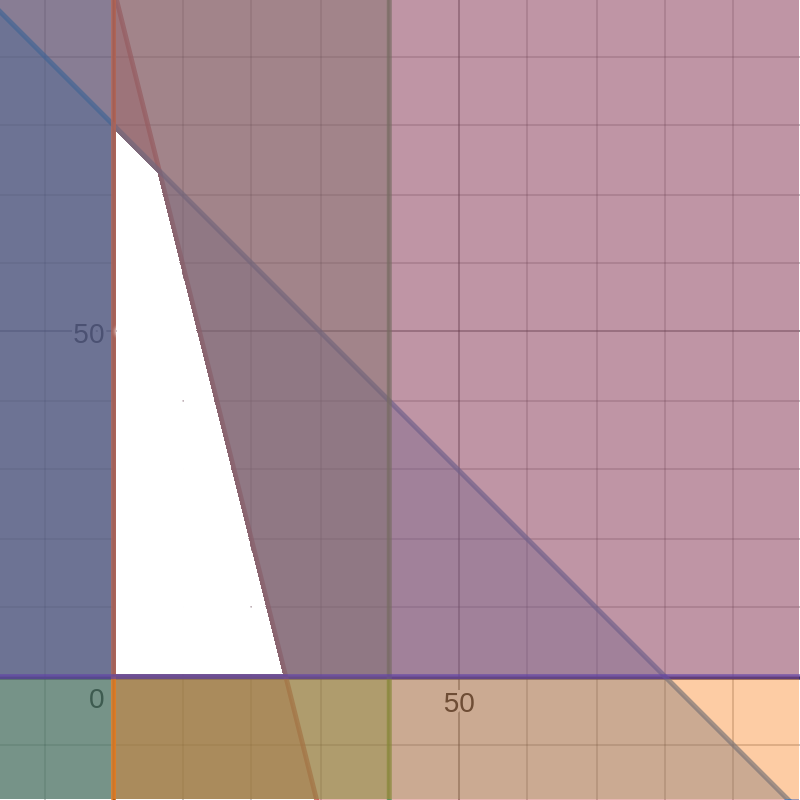
\includegraphics[height=1\textwidth]{graph1.png}
\caption{Feasible Set ( Painted White) }
\end{figure}

\subsection*{b. }
We can  see clearly from the graph that all the intersections between the other constraints occur on the interior of the inequality $x_1 \leq 40$, the area shaded green.
Note that every point along the edge of this inequality is infeasible, and this linear program is degenerate.

\subsection*{c.}
\begin{equation*}
\begin{alignedat}{3}
&\text{max }&z&\\
&\text{s.t. } &z - x_1 - x_2 &= 0 \\
& &4x_1 + x_2 + s_1 &= 100\\
& &x_1 + x_2 + s_2 &= 80\\
& &x_1, x_2, s_1, s_2 &\geq 0
\end{alignedat}
\end{equation*}

We may now construct the matrix to impliment the simplex method.
\[
	\left[ {\begin{array}{ccccc|c}
	Z & x_1 & x_2 & s_1 & s_2 & RHS\\ \cline{1-6}
	1 & -1 & -1 & 0 & 0 & 0 \\
	0 & 4 & 1 & 1 & 0 & 100 \\
	0 & 1 & 1 & 0 & 1 & 80 \\
	\end{array} } \right]
\]
We will pivot on $x_1$. The minimum ratio is the row corresponding to $s_1$. By applying row operations we arrive at:
\[
	\left[ {\begin{array}{ccccc|c}
	Z & x_1 & x_2 & s_1 & s_2 & RHS\\ \cline{1-6}
	1 & 0 & \frac{-3}{4} & \frac{1}{4} & 0 & 25 \\
	0 & 1 & \frac{1}{4} & \frac{1}{4} & 0 & 25 \\
	0 & 0 & \frac{3}{4} & \frac{-1}{4} & 1 & 55 \\
	\end{array} } \right]
\]
Now pivoting on $x_2$ The minimum ratio is the row corresponding to $s_2$. Via row operations:
\[
	\left[ {\begin{array}{ccccc|c}
	Z & x_1 & x_2 & s_1 & s_2 & RHS\\ \cline{1-6}
	1 & 0 & 0 & 0 & 1 & 80 \\
	0 & 1 & 0 & \frac{1}{3} & \frac{-1}{3} & \frac{20}{3} \\
	0 & 0 & 1 & \frac{-1}{3} & \frac{4}{3} & \frac{220}{3} \\
	\end{array} } \right]
\]

We have now reached a solution where: $x_1 = \frac{20}{3}, x_2 = \frac{220}{3}, s_1 = s_2 = 0$
The maximum for this function is now: 80

\subsection*{d.}
Step one began at the basic feasible solution of $(0,0,100,80)$ located at the origin of the graph. The algorithm moved us to
$(25, 0, 0, 55)$ Which is located along the x axis. The next step took us the optimal, located at: $(\frac{20}{3},\frac{220}{3},0,0)$.

\section*{Question 3}

\begin{equation*}
\begin{alignedat}{3}
&\text{max }&z&\\
&\text{s.t. } &z - 2x_1 + 5x_2 &= 0 \\
& &3x_1 + 8x_2 + s_1 &= 12\\
& &2x_1 + 3x_2 + s_2 &= 6\\
& &x_1, x_2, s_1, s_2 &\geq 0
\end{alignedat}
\end{equation*}

\subsection*{a.} 
Note that there are ${4 \choose 2} = 6$ basic solutions to this Linear Program.
\begin{equation*}
\begin{alignedat}{2}
(1) \hspace{1cm}& x_1,x_2 = 0; s_1 = 12, s_2 = 6\\
(2) \hspace{1cm}& x_1,s_1 = 0; x_2 = 12, s_2 = -30\\
(3) \hspace{1cm}& x_1,s_2 = 0; x_2 = 2, s_1 = -4\\
(4) \hspace{1cm}& x_2,s_1 = 0; x_1 = 4, s_2 = -2\\
(5) \hspace{1cm}& x_2, s_2 = 0; x_1 = 3, s_1 = 3\\
(6) \hspace{1cm}& s_1, s_2 = 0; x_1 = \frac{12}{7}, x_2 = \frac{6}{7}
\end{alignedat}
\end{equation*}

\subsection*{b.}
\begin{figure}[H]
\centering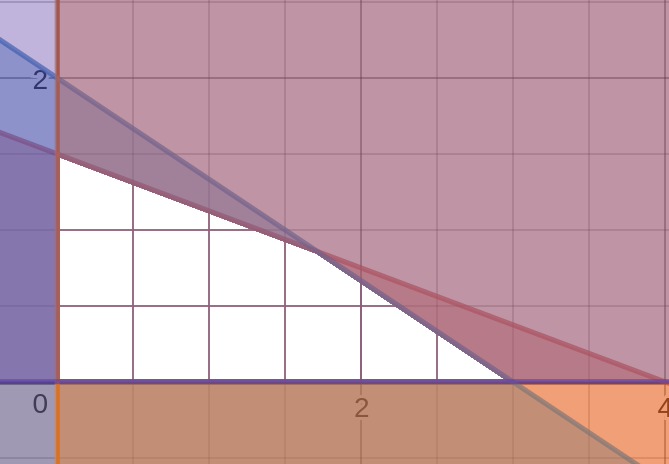
\includegraphics[width=.8\textwidth]{graph2.png}
\caption{Feasible Set ( Painted White) }
\end{figure}

\subsection*{c.}
As we can plainly see, the basic solutions corresponding to (2), (3), (4) are all infeasible. These correspond to intersections of the constraints outside of the feasible set.
Basic solution (1) corresponds to the origin. (5) is the intersection between the blue line and the x-axis. (6) is the intersection between the blue and red lines.

\subsection*{d.}

We may now construct the matrix to impliment the simplex method.
\[
	\left[ {\begin{array}{ccccc|c}
	Z & x_1 & x_2 & s_1 & s_2 & RHS\\ \cline{1-6}
	1 & -2 & 5 & 0 & 0 & 0 \\
	0 & 3 & 8 & 1 & 0 & 12 \\
	0 & 2 & 3 & 0 & 1 & 6 \\
	\end{array} } \right]
\]

We wish to pivot on $x_1$, after conducting the minimum ratio test, we will pivot on the row corresponding to $s_2$.

\[
	\left[ {\begin{array}{cccccc}
	Z & x_1 & x_2 & s_1 & s_2 & RHS\\ \cline{1-6}
	1 & 0 & 8 & 0 & 1 & 6 \\
	0 & 0 & \frac{7}{2} & 1 & \frac{-3}{2} & 3 \\
	0 & 1 & \frac{3}{2} & 0 & \frac{1}{2} & 3 \\
	\end{array} } \right]
\]

Since all elements in the Z row are positive, we are now at the optimum. The solution is $(3,0,3,0)$
The maximum obtained is: 6

\subsection*{e.}
The algorithm begins at the point: $(0,0,12,6)$ Corresponding to basic solution (1) at the origin. It then moves along the $x_2$ axis to $(3,0,3,0)$ where it reaches the optimum, corresponding to solution (5). 

\section*{Question 4.}
\begin{equation*}
\begin{alignedat}{3}
&\text{max }&z&\\
&\text{s.t. } &z - 2x_1 + x_2 - x_3 &= 0 \\
& &3x_1 + x_2 + x_3 + s_1 &= 60\\
& &x_1 -x_2 + 2x_3 + s_2 &= 10\\
& &x_1 + x_2 - x_3 + s_3 &=20\\
& &x_1, x_2, s_1, s_2 &\geq 0
\end{alignedat}
\end{equation*}

\[
	\left[ {\begin{array}{ccccccc|c}
	Z & x_1 & x_2 & x_3 & s_1 & s_2 & s_3 & RHS\\ \cline{1-8}
	1 & -2 & 1 & -1 & 0 & 0 & 0 & 0\\
	0 & 3 & 1 & 1 & 1 & 0 & 0 & 60\\
	0 & 1 & -1 & 2 & 0 & 1 & 0 & 10\\
	0 & 1 & 1 & -1 & 0 & 0 & 1 & 20\\
	\end{array} } \right]
\]

We begin by pivoting on $x_1$, the minimum ratio in that column is the row corresponding to: $s_2$.

\[
	\left[ {\begin{array}{ccccccc|c}
	Z & x_1 & x_2 & x_3 & s_1 & s_2 & s_3 & RHS\\ \cline{1-8}
	1 & 0 & -1 & 3 & 0 & 2 & 0 & 20\\
	0 & 0 & 4 & -5 & 1 & -3 & 0 & 30\\
	0 & 1 & -1 & 2 & 0 & 1 & 0 & 10\\
	0 & 0 & 2 & -3 & 0 & -1 & 1 & 10\\
	\end{array} } \right]
\]

Pivot upon column $x_2$ and row $s_3$.

\[
	\left[ {\begin{array}{ccccccc|c}
	Z & x_1 & x_2 & x_3 & s_1 & s_2 & s_3 & RHS\\ \cline{1-8}
	1 & 0 & 0 & \frac{3}{2} & 0 & \frac{3}{2} & \frac{1}{2} & 25\\
	0 & 0 & 0 & 1 & 1 & -1 & -2 & 10\\
	0 & 1 & 0 & \frac{1}{2} & 0 & \frac{1}{2} & \frac{1}{2} & 15\\
	0 & 0 & 1 & \frac{-3}{2} & 0 & \frac{-1}{2} & \frac{1}{2} & 5\\
	\end{array} } \right]
\]
Since all terms in the Z constraint are positive, we are at the optimal solution. This solution is: $(15, 5, 0, 10, 0, 0)$ The maximum is: 25

\end{document}